\documentclass{llncs}
%\pagestyle{headings} %page numbers
%\usepackage[font=small,labelfont=bf]{caption}


%% Language and font encodings
\usepackage[english]{babel}
\usepackage[utf8x]{inputenc}
\usepackage[T1]{fontenc}
\usepackage[outdir=./]{epstopdf}
\usepackage{bm}
\usepackage{float}

\usepackage[]{xcolor}
%% Sets page size and margins
\usepackage[a4paper,top=3cm,bottom=2cm,left=3cm,right=3cm,marginparwidth=1.75cm]{geometry}

%% Useful packages
%\usepackage{amsmath}
\usepackage{graphicx}

\usepackage[colorinlistoftodos]{todonotes}
\title{Optimized average-based embeddings for word sense disambiguation problem}
\author{Grzegorz Beringer \and Mateusz Jabłoński \and Piotr Januszewski \and Julian Szymański}
%

 \institute{
Faculty of Electronic Telecommunications and Informatics\\
Gda{\'n}sk University of Technology, Gda{\'n}sk, Poland
}

% (feature abused for this document to repeat the title also on left hand pages)

% the affiliations are given next; don't give your e-mail address
% unless you accept that it will be published
%\institute{Faculty of Electronics,
%Telecommunications and Informatics,
%Gdańsk University of Technology,
%ul. Narutowicza 11/12, 80-952 Gdańsk,
%Poland}

\begin{document}
\maketitle
\begin{abstract}

In recent years word embeddings have been shown to boost the performance in NLP tasks such as syntactic parsing or sentiment analysis, but also in multimodal systems like image captioning or visual question answering.
It is therefore not surprising that word embeddings have been applied to Word Sense Disambiguation (WSD) problem as well.
In this work, we present how a simple word embeddings average-based method can be used to produce keyword (meaning) and context embeddings, and how the former can be improved with two embeddings distance optimization techniques.
We also open source the dataset that was created for the purpose of this research.
It is composed of 6 ambiguous words, with 4 to 7 meanings each, and collected real-world usage examples of those meanings, with tagged words to be disambiguated.

\keywords{word sense disambiguation, word embeddings}
\end{abstract}

\section{Introduction}
\label{introduction}

Word Sense Disambiguation (WSD) is an open problem of natural language processing (NLP) and ontology. WSD is identifying which sense of a word (i.e. meaning) is used in a sentence based on the word context. Difficulty is when the word has multiple meanings (e.g. a decision tree, a tree data structure, a tree in a forest). The problem requires two inputs: a dictionary to specify the senses which are to be disambiguated and a corpus of language data to be disambiguated. WSD task has two variants: "lexical sample" and "all words" task. The former aim to disambiguate the occurrences of a small sample of selected target words, while in the latter all the words in a piece of running text need to be disambiguated. Our solution targets the former one, but could be extended to the latter variant.
The solution to WSD would be useful in many NLP related problems as: relevance of search engines, anaphora resolution, coherence, inference, etc.

Word embeddings are a product of feature learning techniques in NLP, where words from the vocabulary are mapped to vectors of real numbers. Conceptually it involves a dimensionality reduction from a space with one dimension per word to a continuous vector space with a much lower dimension.
Methods to generate this mapping include artificial neural networks\cite{word2vec}\cite{GloVe}\cite{fastText}, dimensionality reduction on the word co-occurrence matrix\cite{Levy2014NWE} and probabilistic models\cite{Globerson2007EEC}.
Word embeddings are commonly used as the input representation. They have been shown to boost the performance in NLP tasks such as syntactic parsing\cite{parsingGrammars} and sentiment analysis\cite{sentimentAnalysis}.

Word embeddings cannot distinguish between different meanings of ambiguous words by themselves. By definition, there is only one embedding for each word e.g. for word ``tree'' there is a single real-valued vector. What can be done, is to try to distinguish the meaning based on the context, in which the word was used. Then, we treat each meaning as a separate keyword, which has its own embedding.
We propose a simple method to infer the word meaning: an average of the context and the word embeddings and number of improvements to this approach in the chapter ``Our method''. Experiments with our solution are presented in the chapter ``Experiments''. To conduct those experiments we have created the dataset composed of 6 ambiguous words, with 4 to 7 meanings each, and collected real-world usage examples of those meanings, with tagged words to be disambiguated. We describe our dataset in the chapter ``Dataset''. In the chapter ``Related work'' we present other approaches to WSD.

\section{Related work}
\label{related work}

Typically, there are two kinds of approach for WSD: supervised, which make use of sense-annotated training data, and knowledge-based, which make use of the properties of lexical resources. In supervised approach, the most widely used training corpus used is SemCor\cite{semcor}, with 226,036 sense annotations from 352 manually annotated documents.
Knowledge-based systems usually exploit WordNet\cite{wordnet} or BabelNet\cite{babelnet} as semantic network.
Our solution joins two approaches. We use the knowledge-based word embeddings like GloVe\cite{GloVe} as a baseline for our method and then optimize them in supervised fashion.

The most usual baseline is the Most Frequent Sense\cite{evalmfs} (MFS) heuristic, which selects for each target word the most frequent sense in the training data.
Recent growth of sequence learning techniques using artificial neural networks contributed to WSD research: Raganato et al.\cite{neuralseqmodelingforWSD} propose a series of end-to-end neural architectures directly tailored to the task, from bidirectional Long Short-Term Memory (LSTM) to encoder-decoder models. Melamud et al.\cite{context2vec} also use bidirectional LSTM it their work. They use large plain text corpora to learn a neural model that embeds entire sentential contexts and target words in the same low-dimensional space, which is optimized to reflect inter-dependencies between targets and their entire sentential context as a whole.

Iacobacci et al.\cite{embeddingsforWSD} were first to try to use word embeddings for WSD. They consider four different strategies for integrating a pre-trained word embeddings as context representation in a supervised WSD system: concatenation, average, fractional and exponential decay of the vectors of the words surrounding a target word.
Peters et al.\cite{deepcontext} create word representations that differ from traditional word embeddings in that each token is assigned a representation that is a function of the entire input sentence. They use vectors derived from a bidirectional LSTM that is trained with a coupled language model objective on a large text corpus.

Most of the previous neural networks applications to WSD ignore lexical resources like glosses (sense definitions) and rely solely on word's context. In Luo et al.\cite{glosses} paper, they integrate the context and glosses of the target word into a unified framework, in order to make full use of both labeled data and lexical knowledge.

Entity Linking (EL) and WSD both address the lexical ambiguity of language. The aim of EL is to discover mentions of entities within text and to link them to the most suitable entry in a reference knowledge base. The two tasks are pretty similar, but they differ fundamentally: in EL the textual mention can be linked to a named entity which may or may not contain the exact mention, while in WSD there is a perfect match between the word form and a suitable word sense in the knowledge base.
Moro et al.\cite{babelfy} present Babelfy, a unified graph-based approach to EL and WSD based on a loose identification of candidate meanings coupled with a densest subgraph heuristic, which selects high-coherence semantic interpretations.
We can find also application of random walks\cite{randomwalks} and topic models\cite{topicmodels} for knowledge-based WSD.

Developing WSD system requires much effort and as a result, very few open source WSD systems are publicly available. Zhong et al.\cite{itmakessense} present an English all-words WSD system, IMS (It Makes Sense), built using a supervised learning approach that is written in Java and completely open source. Following Lee and Ng\cite{SVMtoWSD}, they adopt support vector machines (SVM) as the classifier and integrate multiple knowledge sources including parts-of-speech (POS), surrounding words, and local collocations as features.

\section{Dataset}
\label{sec:dataset}
For the purpose of testing word embeddings as a method to differentiate between different meanings, we gathered examples for 6 ambiguous words, 4-7 meanings each (28 meanings in total).
Ambiguous word together with its meaning constitues a \textit{keyword}, which we use as a separate class when identyfing the closest meaning given some context.
All keywords can be seen on Fig. \ref{fig:keywords}.

\begin{figure}
    \centering
    \caption{Ambiguous words with their meanings that are present in the dataset. Each word-meaning pair is called a keyword, e.g. \textit{tree forest}, \textit{pool computer science}.}
    \label{fig:keywords}
    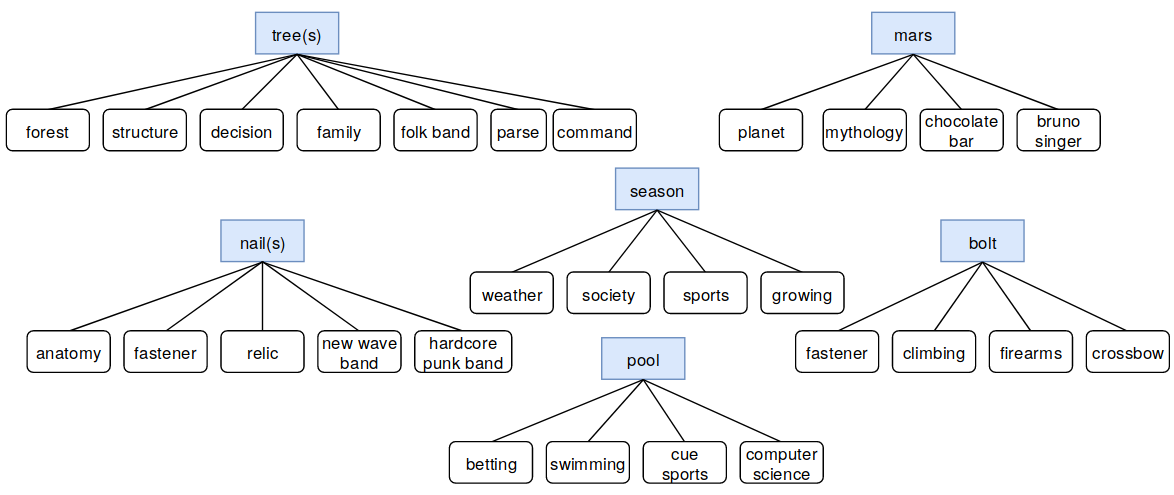
\includegraphics[scale=0.35]{res/keywords.png}
\end{figure}

Examples were mostly gathered from Wikipedia, using \textit{What links here} utility for each keyword.
If usage examples from Wikipedia were not enough, other websites were used (or even the Wikipedia article on specific keyword itself).

The dataset is split into training and test set, with 5 training and 10 test examples for each keyword.
Each example is stored in plain text, with the ambiguous word marked with "*" on both sides.

The correct keyword for each example, together with a path to file and a link, where the original text was taken from, are stored in CSV files: \textit{train.csv} for training set, \textit{test.csv} for test set (columns: path,keyword,link).
Keywords themselves, together with links to their Wikipedia articles, are stored in \textit{keywords.csv} file.
Dataset, together with the code to execute experiments from this paper, can be found on our GitHub repository \cite{repository}.

\bigskip
\underline{Example for \textit{bolt crossbow} keyword:}

\smallskip
\textbf{Keyword definition}: keyword.csv\newline
\textit{
keyword,link\newline
...\newline
bolt crossbow,https://en.wikipedia.org/wiki/Crossbow\_bolt}

\smallskip
\textbf{Test set}: test.csv\newline
\textit{
path,keyword,link\newline
...\newline
texts/test/bolt\_crossbow\_5.txt,bolt crossbow,https://en.wikipedia.org/wiki/Incendiary\_device
}

\smallskip
\textbf{Text}: texts/test/bolt\_crossbow\_5.txt\newline
\textit{"Sulfur- and oil-soaked materials were sometimes ignited and thrown at the enemy, or attached to spears, arrow and *bolts* and fired by hand or machine. Some siege techniques—such as mining and boring—relied on combustibles and fire to complete the collapse of walls and structures."}

\section{Our method}
\subsection{Keyword embedding}
\label{sec:kw_embed}
\textit{Keyword} is a sequence of words that lets us disambiguate between different meanings of the same ambiguous word, e.g. "tree forest" that represents a tree as a plant and "tree structure" which represents tree as a mathematical structure.

To get the embedding of the keyword, we simply average all the words in the keyword:

\begin{equation}
    \label{eq:keyword_embedding}
    \bm{k} = e(w_1, w_2, ..., w_N) = \frac{1}{N}\sum_{i=1}^{N} e(w_i)
\end{equation}

where \(e(\cdot)\) is the embedding function used and \(w_1, w_2, ..., w_N\) is a sequence of N words that, in this case, constitutes a keyword.

\subsection{Context embedding}
\label{sec:ctx_embed}
\textit{Context} is a sequence of words that contains an ambiguous word within, usually in the middle.
It is parametrized by context length \(l\), which specifies how many of words from both side of the ambiguous word in question were taken into consideration.

\textit{Context embedding} \(\bm{c}\) is also achieved by taking an average of word embeddings (Equation \ref{eq:keyword_embedding}).
In this case, \(N = 2l + 1\) and \(w_1, w_2, ..., w_N\) is the context with ambiguous word inside. For some cases \(N < 2l + 1\), since the ambiguous word may occur at the beginning or ending of text example and full context cannot be collected.
In this case, we just average the reduced context.

Text, that we take context from, must be preprocessed.
We remove any special characters and stopwords, and use lower-case letters only.

\underline{Example with \(l=3\)}:

\textbf{Text}:
\textit{"The object pool pattern is a software creational design pattern that uses a set of initialized objects kept ready to use – a " *pool* " – rather than allocating and destroying them on demand."}

\textbf{Preprocessed text}:
\textit{"the object pool pattern is a software creational design pattern that uses a set of initialized objects kept ready to use a *pool* rather than allocating and destroying them on demand"}

\textbf{Context}:
\textit{kept ready use \underline{pool} rather allocating destroying}

\subsection{Optimization}
\label{sec:optimization}
As a baseline, we use keyword and context embeddings described above to find the closest keyword given some context, using cosine distance as a metric.
To optimize this system, we use texts from the training set to improve the quality of keyword embeddings.
For each training example, we shift the correct keyword embedding by a factor of \(\alpha\) in the direction of context embedding, which describes said keyword.

\begin{equation}
    \label{eq:alpha_optimization}
    \bm{k}^{(i+1)} = \bm{k}^{(i)} + \alpha(\bm{c} - \bm{k}^{(i)})
\end{equation}

where \(\bm{k}^{(i)}\) is the embedding of the correct keyword at iteration \(i\), \(\bm{c}\) is the context embedding and \(\alpha\) is a scalar that controls the strength of the update.

\smallskip
We try to optimize the system even further, by also moving top-k closest keywords that are incorrect given the same context.

\begin{equation}
    \label{eq:beta_optimization}
    \bm{m}^{(i+1)} = \bm{m}^{(i)} - \beta(\bm{c} - \bm{m}^{(i)})
\end{equation}

where \(\bm{m}^{(i)}\) is the embedding of incorrect keyword at iteration \(i\) and \(\beta\) is a scalar that controls the strength of the update.

\subsection{Limitations}
\label{sec:limitations}
We are aware that our method has some limitations.
First of all, it may be impossible to achieve the optimal solution, as we can only optimize keyword embeddings, leaving context embeddings fixed in the multidimensional space.
Therefore, it is possible that contexts for specific keyword overlap on contexts for other keyword.

Secondly, the average context embedding may be ambiguous, with a high possibility of two different context being mapped to a similar point in space, especially for longer context legths.
In future work (\ref{sec:conclusion}), we suggest experimenting with different sequence embedding techniques, that might be better suited for this purpose than a flat average.


\section{Experiments}
The goal of following experiments is to check how embedding approach (\ref{sec:kw_embed}, \ref{sec:ctx_embed}) works for the dataset we collected (\ref{sec:dataset}), both out-of-the-box (baseline) and after applying optimization techniques (\ref{sec:optimization}).
We use a pretrained embedding model from spaCy - \textit{en\_vectors\_web\_lg}, which contains 300-dimensional word vectors trained on Common Crawl with GloVe\cite{spacymodel}.

Due to the high impact of training data order on test results, we take the average score of 30 runs (each with a random order of training data) for each optimization experiment.
The best configuration of each experiment is taken as a baseline for the next experiment.
The goal of these experiments is to show how each of parameters influences on model's accuracy after training.

We compare results on the test set with two metrics: top-1 accuracy, where we are only interested, if the correct keyword is the closest one to a specific context describing it, and top-3 accuracy, where we check if we are in the closest three keywords.

\subsection{Baseline}
\label{sec:baseline}
For the baseline model, we check how out-of-the-box keyword (\ref{sec:kw_embed}) and context embeddings (\ref{sec:ctx_embed}) work without any extra optimizations.
We evaluate the performance of the model with different context lengths, to see how it affects top-1 and top-3 accuracies (Fig. \ref{fig:baseline}).

\begin{figure}[H]
    \centering
    \caption{Top-1 and top-3 accuracies of the baseline model with different context lengths.}
    \label{fig:baseline}
    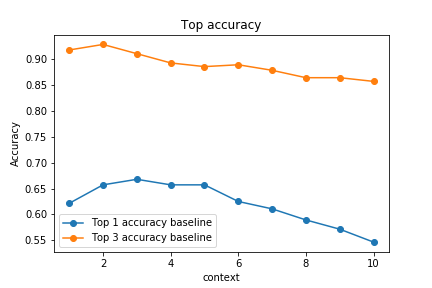
\includegraphics[scale=0.5]{res/baseline_context_top_acc.png}
\end{figure}

We can see, that the model does relatively well, even unoptimized.
Top-3 accuracy is about 85-90\%, which is probably caused by a low number of meanings for each ambiguous word.
Top-1 accuracy for shorter context lengths can go as high as 65\% but decreases with longer contexts.
As suspected (\ref{sec:limitations}), this is most likely due to the fact, that the average of many word embeddings may make some contexts similar to each other, therefore making it harder to distinguish between some meanings.

The best result w.r.t. top-1 accuracy was achieved with \(l=3\), which is why we choose this context length as a starting point for next experiments.

\subsection{Alpha optimization}
\label{sec:exp_alpha}
We check, how a simple optimization method of moving keyword embeddings closer to the contexts they appear in (Eq. \ref{eq:alpha_optimization}), affects the accuracy of the model.
To do this, we arbitrarily choose some \(\alpha\) value (here 0.2), test the results of improved keyword embeddings with different context lengths and compare them to the baseline (\ref{sec:baseline}). Since we average the results from 30 runs, we mark the measurement uncertainty on the graph (Fig. \ref{fig:exp1_optimization}).

\begin{figure}[H]
    \centering
    \caption{Comparison of the baseline model (\ref{sec:baseline}) and a model optimized with \(\alpha=0.2\) for different context lengths.}
    \label{fig:exp1_optimization}
    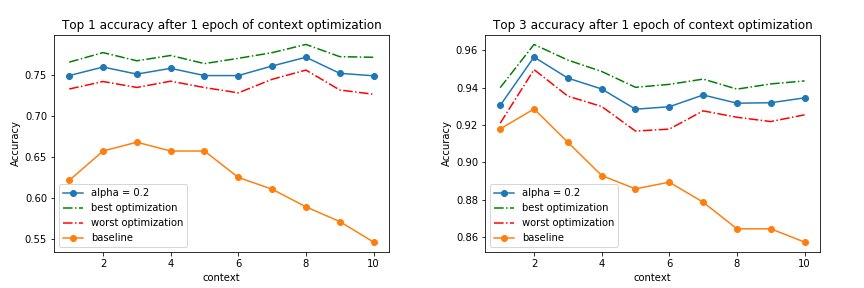
\includegraphics[scale=0.6]{res/exp1_context_top_acc.png}
\end{figure}

Independently of some noise caused by the random order of training data, the optimized model is much better than the base model (12-36\% relative, 10-20\% absolute improvement w.r.t. top-1 accuracy on the test set).
Improvement is most visible for longer context lengths, which achieved relatively poor results in the baseline experiment.
It seems, that a simple optimization may help alleviate the problems with ambiguous embeddings of long contexts (\ref{sec:limitations}).

Overall, results suggest, that for an optimized model, context length is not as important as with the baseline model, at least with this particular \(\alpha\) value.

\bigskip
Next, we check the influence of the \(\alpha\) parameter value on the top-1 and top-3 accuracies for \(l=3\) (Fig. \ref{fig:exp2_alpha}).

\begin{figure}[H]
    \centering
    \caption{Influence of \(\alpha\) parameter value on top-1 and top-3 accuracies for \(l=3\). Blue line denotes the average result from 30 runs, dotted lines denote worst and best result. The value for \(\alpha=0\) is the result achieved by the baseline model (\ref{sec:baseline}).}
    \label{fig:exp2_alpha}
    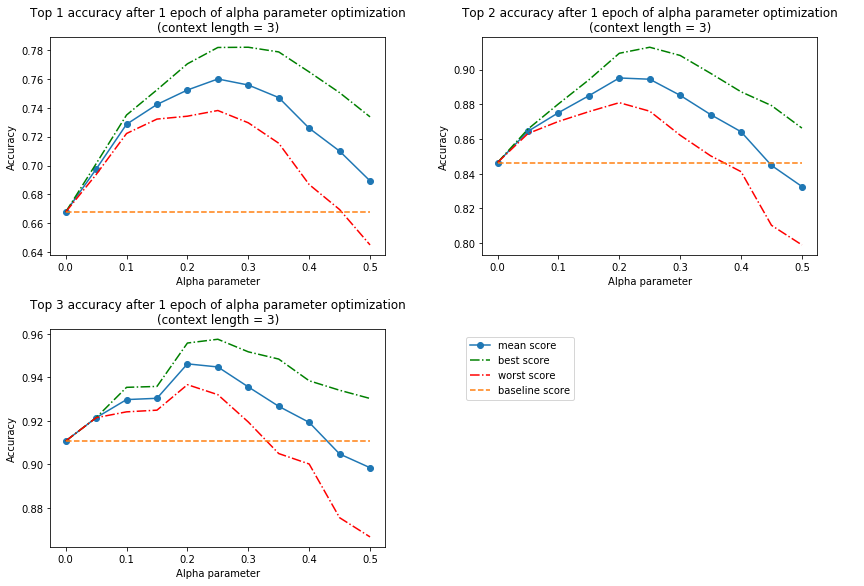
\includegraphics[scale=0.6]{res/exp2_alpha_top_acc.png}
\end{figure}

Top-1 accuracy grows up to \(\alpha=0.25\) and then starts to drop.
It suggests, that bigger values of \(\alpha\) may cause the movement on the multidimensional plane to be too chaotic, moving the correct keyword embedding too close to a specific context, causing overfitting to a specific example.
Similarly, small values of \(\alpha\) may update the keyword embedding too little, ending up in only slightly better position.

\subsection{Beta optimization}
We proved that moving keyword embeddings closer to their contexts is beneficial for the accuracy on the test set (\ref{sec:exp_alpha}).
We theorize, that the results could be further improved, if we also increase the distance between closest incorrect keyword embeddings and the context embedding for a specific example (Eq. \ref{eq:beta_optimization}).

In following experiment, we therefore check the influence of \(\beta\) parameter value on the accuracy on the test set, for \(l=3, \alpha=0.25\) (Fig. \ref{fig:exp3_beta}).
Since we compare the results to an average value from previous experiments (Fig. \ref{fig:exp2_alpha}), we decide to only plot an average result achieved by this optimization.

\begin{figure}[H]
    \centering
    \caption{Influence of \(\beta\) parameter value on top-1 and top-3 accuracies for \(l=3\) nad \(\alpha=0.25\). The value for \(\beta=0\) is the best result achieved by the model from previous experiment (Fig. \ref{fig:exp2_alpha}).}
    \label{fig:exp3_beta}
    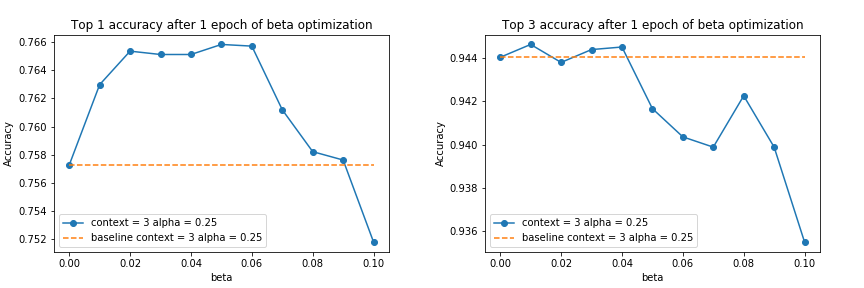
\includegraphics[scale=0.6]{res/exp3_beta_top_acc.png}
\end{figure}

Low values of \(\beta\) seem to slightly improve the performance of our optimization method w.r.t. top-1 accuracy (about 1\% absolute and relative improvement).
High values of \(\beta\) suffer from a similar problem to high values of \(\alpha\), causing too much disruption to keyword embeddings.

We chose to move only top-3 closest keywords per each training example. In future work, it might be interesting to see, how does the number of keyword embeddings moved affects the results. We also theorize, that influence of this particular optimization could be bigger for trainings with more than 1 epoch.

\subsection{Accuracy in time}
In previous experiments, we passed through the training data only once, which may not be optimal.
The goal of this experiment is to check how a number of epochs (full passes through training data) affects the final accuracy.
We run 5 epochs of training, using best parameters from previous experiments: \(l=3, \alpha=0.25, \beta=0.05\) (Fig. \ref{fig:exp4_1_epochs_fixed}).

\begin{figure}[H]
    \centering
    \caption{Top-1 and top-3 accuracy for model with \(l=3, \alpha=0.25, \beta=0.05\) trained for 5 epochs.}
    \label{fig:exp4_1_epochs_fixed}
    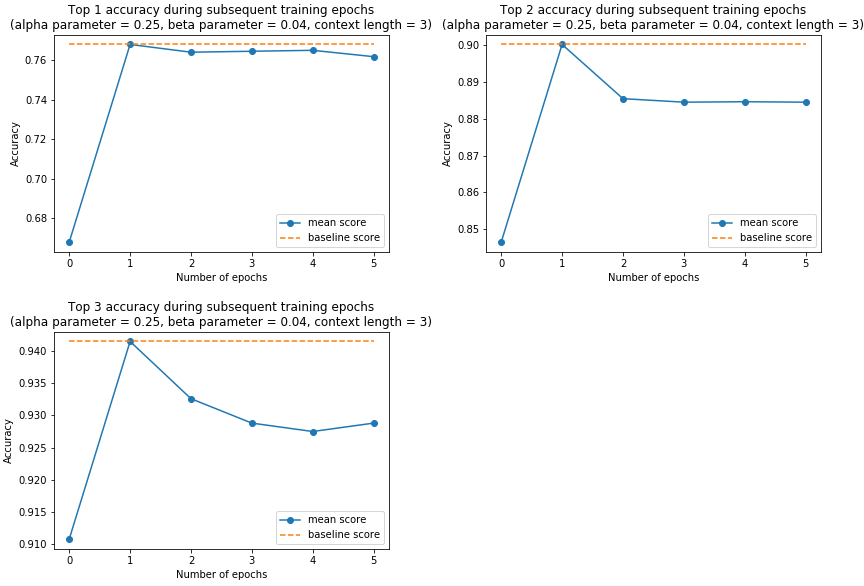
\includegraphics[scale=0.6]{res/exp4_epoch_top_acc.png}
\end{figure}

We see that there is almost no improvement after the first epoch of training.
The possible problem is that the values of \(\alpha\) and \(\beta\) are too high, causing the updates to keyword embeddings to be too big.
We therefore check what happens, when we choose lower values of these parameters (Fig. \ref{fig:exp4_2_epochs_comparison}).

\begin{figure}[H]
    \centering
    \caption{Comparison of models optimized with different \(\alpha\) and \(\beta\) values with \(l=3\) for 5 epochs.}
    \label{fig:exp4_2_epochs_comparison}
    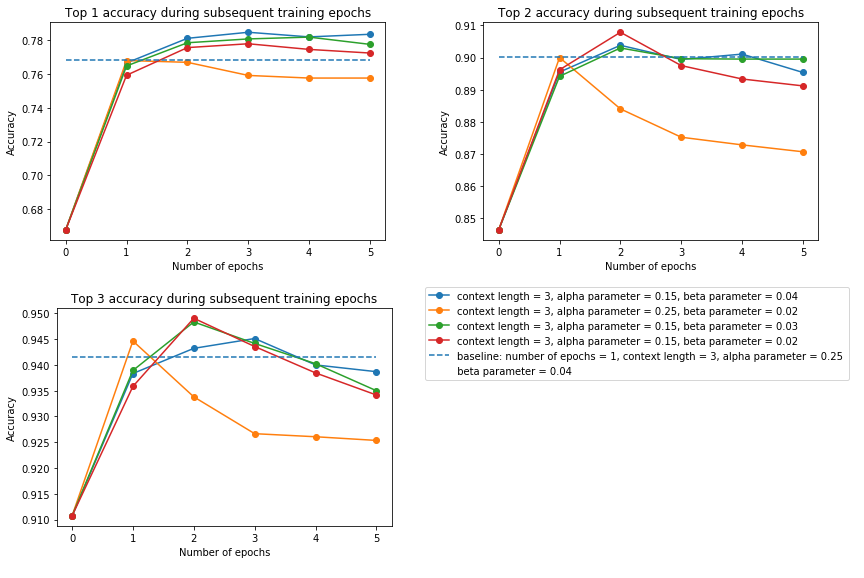
\includegraphics[scale=0.6]{res/exp4_epoch_multiconfiguration_top_acc.png}
\end{figure}

Longer training shows that optimal parameters obtained from previous experiments are not necessarily good for multiple passes through the training data.
If we train for a bigger number of epochs, lower values of \(\alpha\) and \(\beta\) parameters are better.
In future work (\ref{sec:conclusion}) we suggest, that a decay parameter might be useful for this particular reason, with each update being a bit smaller to fine-tune the results.


\section{Conclusion and future work}
\label{sec:conclusion}

Average-based keyword and context embeddings proved to be a surprisingly good baseline for the dataset of ambiguous keywords that we collected, achieving over 65\% top-1 and 93\% top-3 accuracy.
We have shown, that you can improve these results up to about 79\% top-1 and 95\% top-3 accuracy by using a simple optimization method of improving keyword embeddings with even a few training examples per keyword.

Further improvements could be sought by using different keyword and context embedding schemes, e.g. weighted average or by using some sentence embedding method. Optimization method itself could be made more stable by applying decay to alpha and beta parameters and by using a validation set for early stopping. It could also be bound to cosine distance between the keyword and context - the bigger the difference, the bigger the update. Finally, the dataset could be enhanced to contain more ambiguous words and training/test examples.

\bibliographystyle{splncs}
\bibliography{sample}

\end{document}


\begin{thebibliography}

\end{thebibliography}
